\chapter{Projektplanlægning}
Indledningsvis kom vi ind på, at vi har brugt Asana til projektstyring.
På Asana har vi delt projektet op i forskellige \textit{tasks} og uddelegeret opgaverne lige og ladet alle bidrage til alle opgaverne.
Det ses i \ref{fig:Asana}, at programmet er opddelt i tre spalter; \textit{tasks}, \textit{in progress} og \textit{done}, som dynamisk ændrer sig gennem projektforløbet.
\begin{figure}[h]
    \begin{center}
        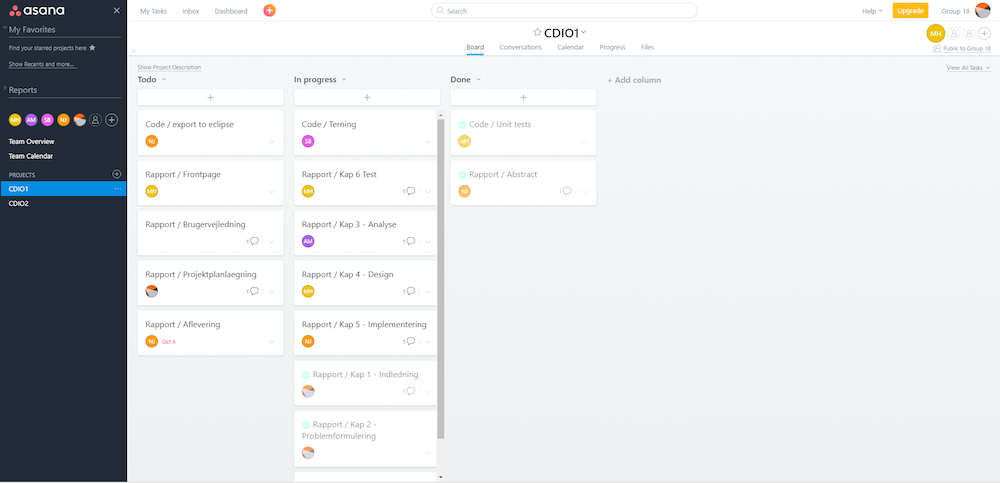
\includegraphics[width=15cm]{graphics/Asana}
        \caption{Screendump af Asana}
    \label{fig:Asana}
    \end{center}
\end{figure}

Asana understøtter UP, idet man kan oprette x-antal tasks som eksempelvis 'inception' og 'elaboration' og derefter lave x-antal \textit{subtasks}, som kan svare til iterationer.